\documentclass{recipe}

\begin{document}
\begin{recipe}{Tuna Cakes}
  \servings{4}

  \begin{ingredients}
    \ingredient{1}{large}{egg}
    \ingredient{1}{can}{tuna}
    \ingredient{1}{slice}{bread}
    \ingredient{\nicefrac{1}{4}}{tbsp}{mustard}
    \ingredient{\nicefrac{1}{4}}{tbsp}{mayonaise}
    \ingredient{}{}{salt}
    \ingredient{}{}{paprika}
    \ingredient{}{}{cayenne pepper}
    \ingredient{}{}{flour}
    \ingredient{}{}{butter}
    \ingredient{}{}{tarter sauce}
  \end{ingredients}

  \begin{images}
    \begin{image}
      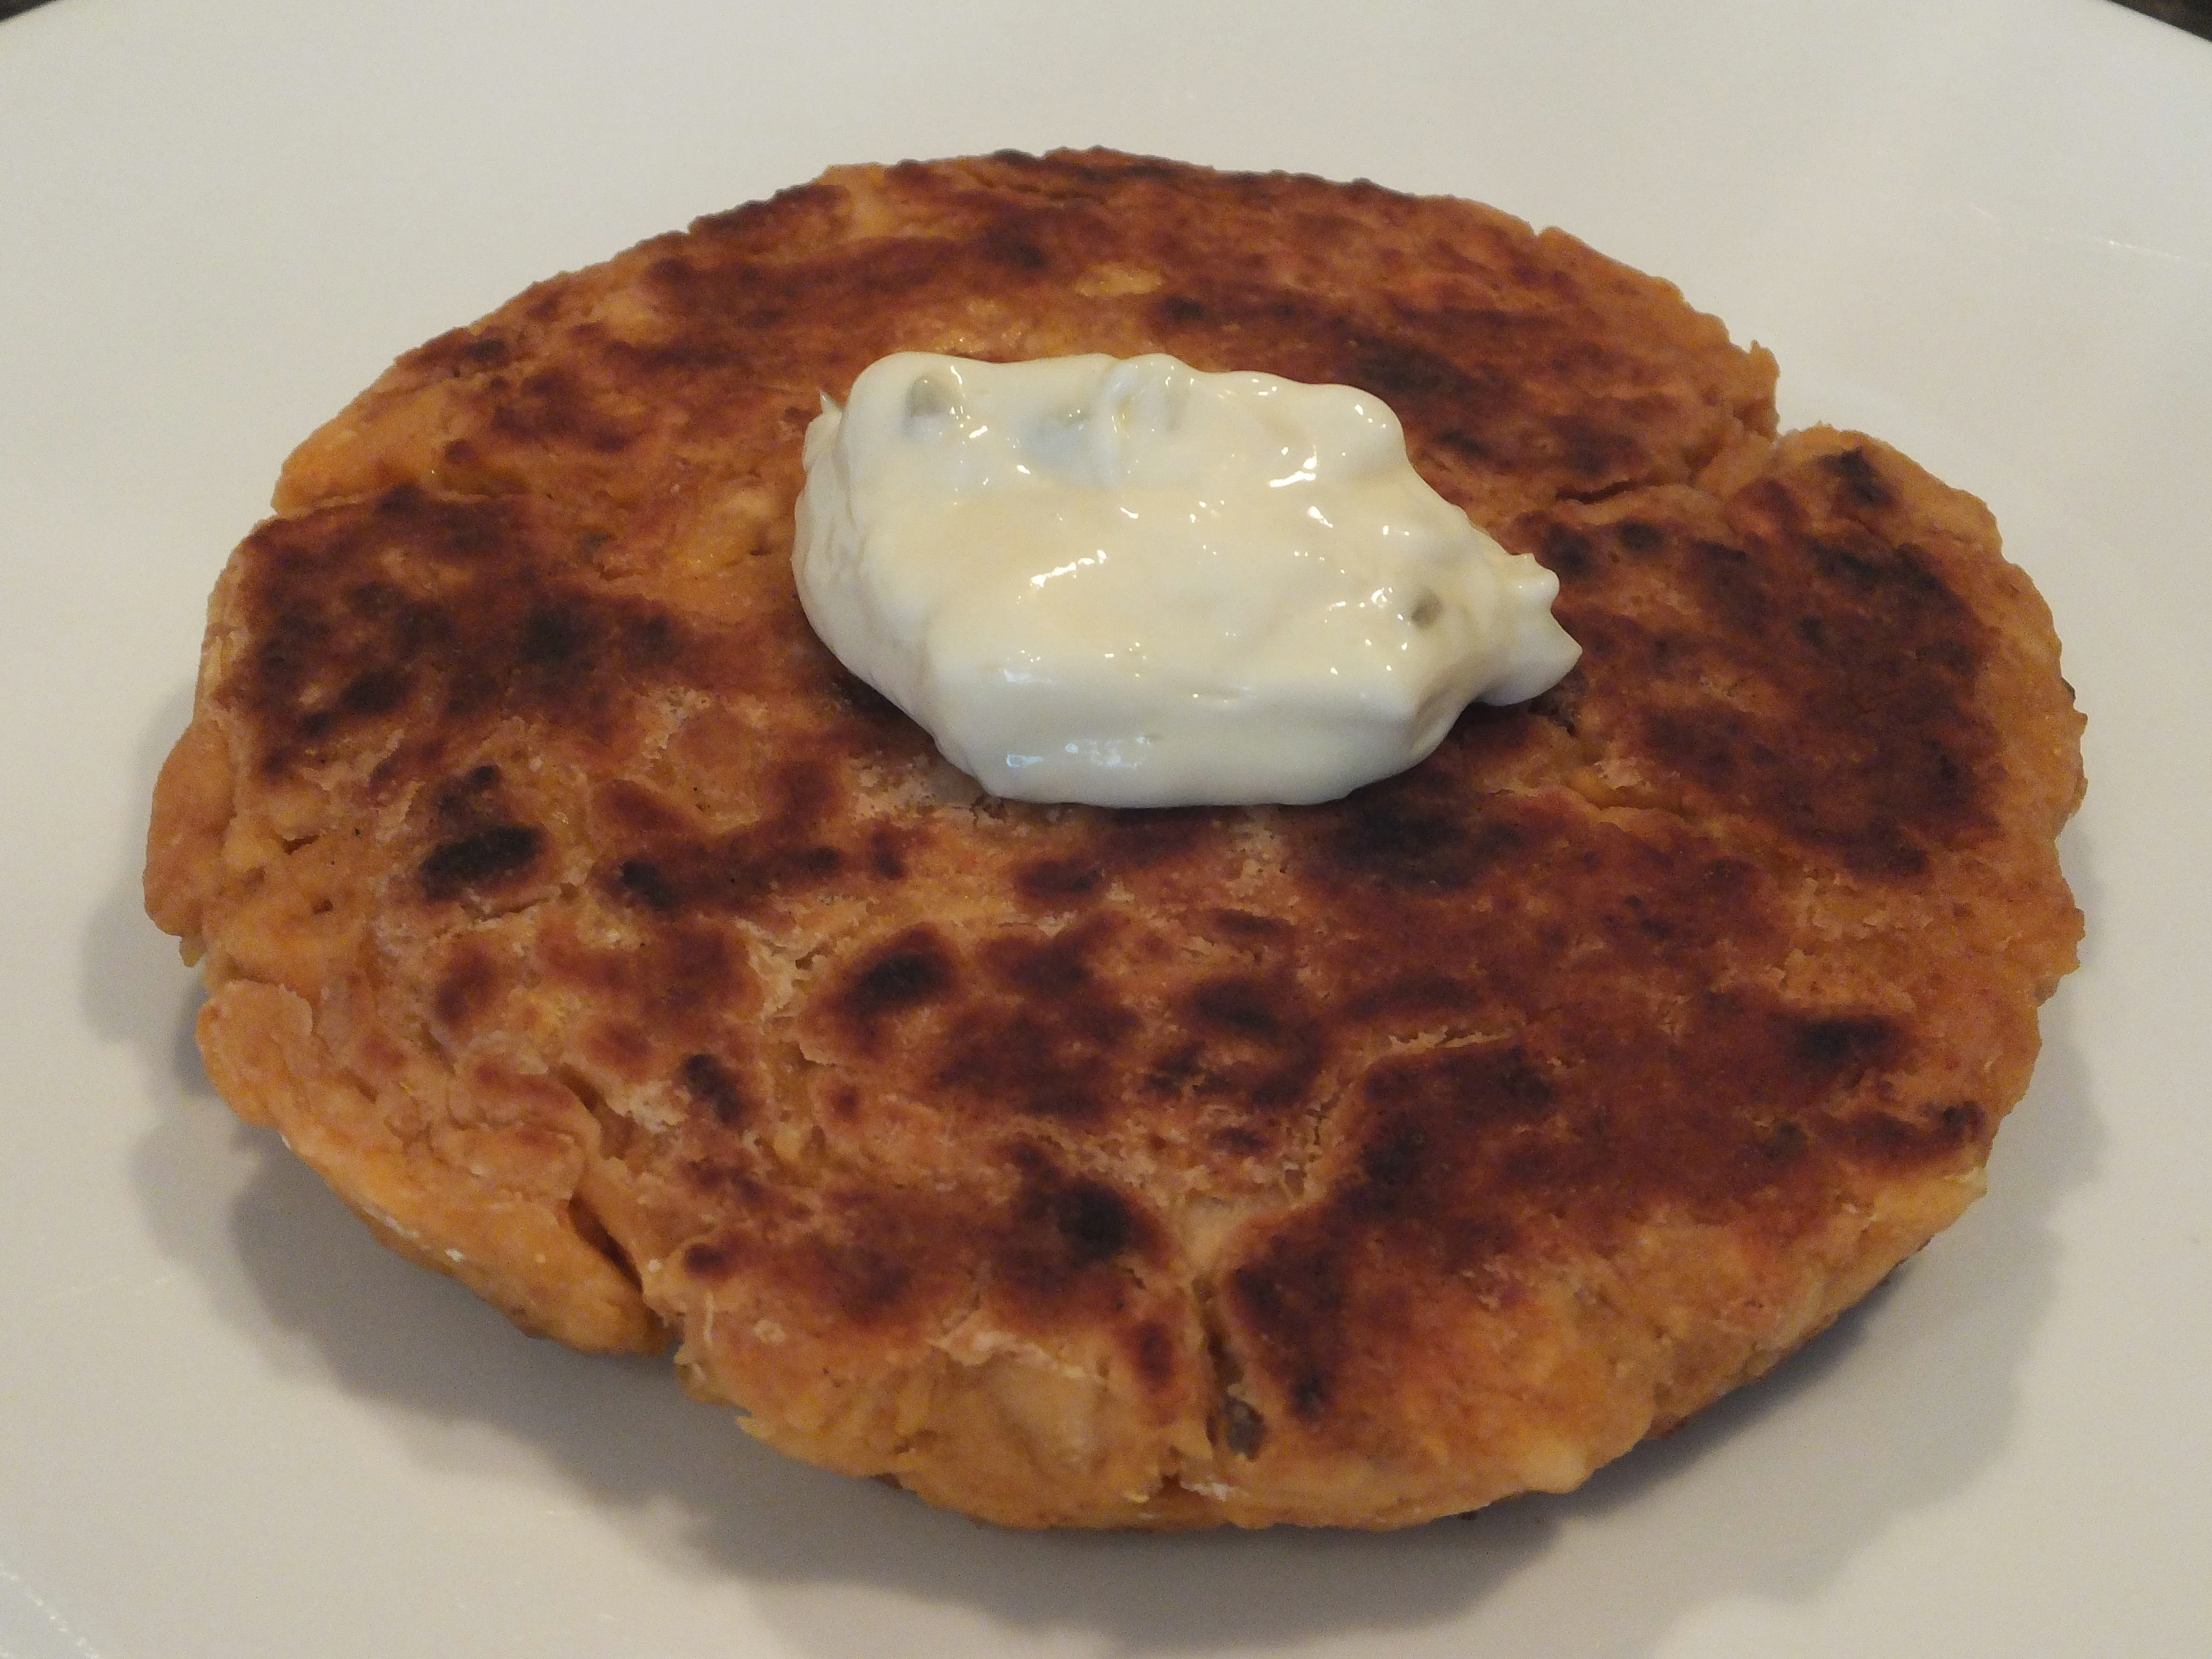
\includegraphics[width=\linewidth,trim=100px 100px 100px 100px, clip=true]{tuna_cakes-01.jpeg}
    \end{image}
  \end{images}

  \begin{steps}
  \item Butterfly and toast the bread
  \item Drain and flake the tuna
  \item Mix the egg, mayonaise, mustard, and dry spices into the tuna
  \item Crumble the toast into the mixture to form a dough
  \item From the dough into the shapes you desire
  \item Dredge the shaped cakes in flour
  \item Fry in butter until brown
  \item Serve with tarter sauce
  \end{steps}

  \begin{notes}
  \item This is pretty much just a crab cake, but with tuna instead!
  \end{notes}
\end{recipe}
\end{document}
